\documentclass{article}

\usepackage{fancyhdr} % Required for custom headers
\usepackage{lastpage} % Required to determine the last page for the footer
\usepackage{amsmath}
\usepackage{amsfonts}
\usepackage{graphicx}
\usepackage{subfigure}
\usepackage{listings}
\usepackage{booktabs}
\usepackage[hidelinks]{hyperref}
% \usepackage{epstopdf} uncomment this line if using MiKTeX

% Margins
\topmargin=-0.45in
\evensidemargin=0in
\oddsidemargin=0in
\textwidth=6.5in
\textheight=9.0in
\headsep=0.25in

\linespread{1.25} % Line spacing

% Set up the header and footer
\pagestyle{fancy}
\lhead{\authorName} % Top left header
\chead{\classID\ \hwTitle} % Top center header
\rhead{\studentID} % Top right header
\lfoot{} % Bottom left footer
\cfoot{} % Bottom center footer
\rfoot{Page\ \thepage\ of~\pageref{LastPage}} % Bottom right footer
\renewcommand{\headrulewidth}{0.4pt} % Size of the header rule
\renewcommand{\footrulewidth}{0.4pt} % Size of the footer rule

\setlength{\parindent}{0pt} % Removes all indentation from paragraphs

\setcounter{secnumdepth}{0} % Removes default section numbers
\newcounter{problemCounter} % Creates a counter to keep track of the number of problems

\newcommand{\problemName}{}
\newenvironment{problem}[1][Problem \arabic{problemCounter}]{
	\stepcounter{problemCounter} % Increase counter for number of problems
	\renewcommand{\problemName}{#1} % Assign \problemName the name of the problem
	\section{\problemName} % Make a section in the document with the custom problem count
}{}

\newcommand{\subproblemName}{}
	\newenvironment{subproblem}[1]{
	\renewcommand{\subproblemName}{#1} % Assign \subproblemName to the name of the section from the environment argument
	\subsection{\subproblemName} % Make a subsection with the custom name of the subsection
}{}

%----------------------------------------------------------------------------------------
%	MATH OPERATOR
%----------------------------------------------------------------------------------------

\DeclareMathOperator*{\argmin}{arg\,min}
\DeclareMathOperator*{\argmax}{arg\,max}

%----------------------------------------------------------------------------------------
%	NAME AND CLASS SECTION
%----------------------------------------------------------------------------------------

\newcommand{\hwTitle}{Assignment\ \#4} % Assignment title
\newcommand{\dueDate}{Thursday,\ April\ 21,\ 2016} % Due date
\newcommand{\classID}{ENGG\ 5202} % Course/Class
\newcommand{\authorName}{Kai Chen} % Your name
\newcommand{\studentID}{1155070509} % Your student ID

%----------------------------------------------------------------------------------------
%	TITLE PAGE
%----------------------------------------------------------------------------------------

\title{
	\vspace{2in}
	\textmd{\textbf{\classID:\ \hwTitle}}\\
	\normalsize\vspace{0.1in}\small{Due\ on\ \dueDate}
	\vspace{3in}
}

\author{\textbf{\authorName}}
\date{} % Insert date here if you want it to appear below your name

%----------------------------------------------------------------------------------------

\begin{document}
\maketitle
\setcounter{page}{0}
\thispagestyle{empty}
\newpage

%----------------------------------------------------------------------------------------
%	PROBLEM 1
%----------------------------------------------------------------------------------------

% To have just one problem per page, simply put a \clearpage after each problem

\begin{problem}

Figure~\ref{fig:1_1} shows the network structure:

\begin{figure}[htbp]
\centering
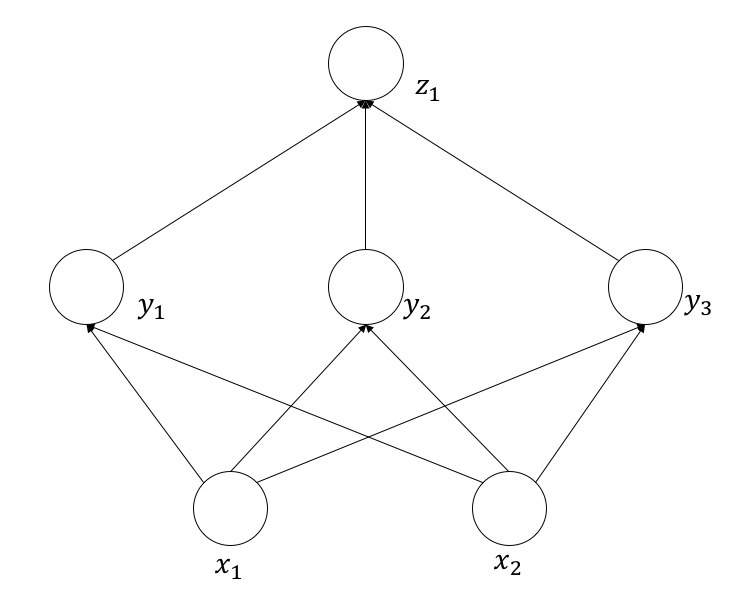
\includegraphics[width=4in]{image/1_1}
\caption{Support vectors of Set1}\label{fig:1_1}
\end{figure}

Nonlinear activation function
\[
f(x) = 
\begin{cases}
1& x\geq0 \\
0& x<0
\end{cases}
\]

Weights are
\begin{align*}
y_1 &= f(x_1 + 1) \\
y_2 &= f(x_2 + 1) \\
y_3 &= f(-x_1 - 2x_2 + 1) \\
z_1 &= f(y_1 + y_2 + y_3 - 2.5)
\end{align*}

\end{problem}

%----------------------------------------------------------------------------------------
%	PROBLEM 2
%----------------------------------------------------------------------------------------

\begin{problem}
\begin{align*}
\frac{\partial J}{\partial w_{kj}} &= \frac{\partial J}{\partial z_k}\frac{\partial z_k}{\partial (net_k)}\frac{\partial (net_k)}{\partial w_{kj}} \\
&= {(t_k - z_k)}^3 \cdot f^\prime(net_k) \cdot y_j
\end{align*}
So that
\[
\Delta w_{kj} = \eta\frac{\partial J}{\partial w_{kj}} = \eta {(t_k - z_k)}^3 \cdot f^\prime(net_k) \cdot y_j
\]
\end{problem}

%----------------------------------------------------------------------------------------
%	PROBLEM 3
%----------------------------------------------------------------------------------------

\begin{problem}

\begin{subproblem}{3.1}
Storage of network parameters: \(O(dn_H + cn_H)\)
Storage of training samples: \(O(nd + n_H + c)\)
Total space comlexity: \(O(dn_H + cn_H + nd)\)
\end{subproblem}

\begin{subproblem}{3.2}
Time complexity is \(O(dn_H+cn_H)\).
\end{subproblem}

\begin{subproblem}{3.3}
Time complexity is \(O(ndn_H+ncn_H)\).
\end{subproblem}

\end{problem}

\end{document}
